\documentclass[11pt]{article}
\usepackage[margin=1in]{geometry}
\usepackage{graphicx,booktabs,amsmath,amssymb,hyperref,caption,subcaption}
% [numbers] puts natbib in numeric mode: the reference list is numbered [1], [2],
% ... and every citation in the text shows its number. \citet still works -- it
% renders as "Karmanov et al. [2]" rather than dropping the number -- so the
% author-year phrasing in the prose survives the switch.
\usepackage[numbers]{natbib}
\graphicspath{{figures/}}
\DeclareMathOperator*{\argmin}{arg\,min}

\title{Calibration-Aware Test-Time Adaptation for CLIP}
\author{Gal Machlin (207627811) \and Idan Yehuda (207016270)}
% Empty, not omitted: dropping \date entirely makes \maketitle print today's
% date, which is the opposite of what is wanted here.
\date{}

\begin{document}
\maketitle

\begin{abstract}
Test-time adaptation (TTA) methods such as TDA~\cite{karmanov2024tda} use only forward
passes and a feature cache to recover much of the accuracy CLIP loses out of distribution, but
a 2025 benchmark~\cite{sheng2025illusion} showed that the gain comes with a hidden cost: TDA's
cache rewards confident predictions whether or not they are correct, so its accuracy gain arrives
bundled with worse calibration (the benchmark reports average ECE rising 5.70\%
$\rightarrow$ 9.21\% across its suite). We propose three training-free, label-free changes to
TDA's cache loop -- margin-based cache admission, probabilistic fusion, and leave-one-out (LOO)
temperature scaling -- meant to recover calibration. Measured on
five datasets (\texttt{ViT-B/16}, test split only), the three changes bundled together as
specified \emph{do not} win: mean accuracy drops from TDA's 56.63\% to 55.22\% and mean ECE
gets \emph{worse}, from 11.24\% to 24.12\%. An ablation isolating each change shows why: two of
the three contributions are actively harmful, and the third -- LOO temperature scaling, run
alone -- is not. It matches the TDA-equivalent baseline's accuracy exactly (56.60\%, to 0.00
points, a structural guarantee of a monotonic rescaling) while cutting mean ECE from 11.28\%
to 8.54\%, a 24\% reduction toward zero-shot CLIP's 5.57\%. We report this honestly: the
bundled method fails, one of its three components alone succeeds, and we explain the
mechanism behind both outcomes.
\end{abstract}

\section{Introduction}

CLIP's zero-shot accuracy is strong on natural-image classification but collapses on
out-of-di\-stri\-bution domains: the benchmark that motivates this project reports 23.7\% on
EuroSAT and 15.7\% on Aircraft~\cite{sheng2025illusion}. Our own zero-shot measurements
(Table~\ref{tab:main}) are higher -- 42.06\% and 23.85\% -- because we evaluate the CoOp test
splits with a \texttt{ViT-B/16} backbone rather than that paper's exact setup; the collapse
relative to in-distribution accuracy is the point, and it reproduces. Test-time adaptation (TTA) methods
close much of this gap without any labels or backpropagation. TDA~\cite{karmanov2024tda}, in
particular, keeps a small cache of features from test images the model is confident about and
reuses that cache to refine later predictions -- a forward-pass-only method with no training
loop.

Accuracy, however, is not the only axis that matters for a system meant to be trusted. A
model that is right 80\% of the time but reports 95\% confidence on every prediction is
\emph{worse} to deploy than one that is honest about its 80\%, because a downstream user or
pipeline has no way to tell a confident-and-correct prediction from a confident-and-wrong one.
This is exactly the failure mode \citet{sheng2025illusion} document in TDA: its cache rewards
confident predictions with more confidence regardless of correctness, so accuracy gains arrive
bundled with a calibration loss (average ECE rising 5.70\% $\rightarrow$ 9.21\% across their
benchmark).

This project asks whether that calibration gap can be closed without retraining and without
labels, by changing three seams of TDA's cache loop:

\begin{enumerate}
    \item \textbf{Margin-based cache admission.} Admit a test sample to the cache by the gap
        between its top-1 and top-2 class scores, instead of by prediction entropy, so the
        cache does not accumulate merely \emph{loud} predictions.
    \item \textbf{Probabilistic fusion.} Combine CLIP's and the cache's evidence as a convex
        mixture of probability distributions, instead of adding raw logits, so agreement
        between the two sources cannot manufacture confidence that neither source had on its
        own.
    \item \textbf{Leave-one-out (LOO) temperature scaling.} Estimate the cache's own accuracy
        without ground truth, via leave-one-out nearest-neighbour agreement among cached
        items, and pick a softmax temperature that makes the model's mean confidence match
        that label-free estimate.
    \end{enumerate}

Each change is independently switchable from configuration, which is what makes the ablation
in Section~\ref{sec:results} possible -- and the ablation is where this project's real finding
lives. \textbf{The three changes together do not improve calibration: they make it
dramatically worse.} Run in isolation, however, one of the three delivers exactly the
calibration improvement this project set out to find, at no accuracy cost. We report both
results without softening either one.

\section{Related Work}

\textbf{Training-free test-time adaptation for CLIP.} TDA~\cite{karmanov2024tda} adapts CLIP
at test time with two small feature caches -- a positive cache keyed by the model's own
predicted class, and a negative cache of low-confidence samples used as a correction term --
built and consumed purely from forward passes, with no backpropagation and no labels. Each new
test image is scored by CLIP and optionally admitted to the positive cache by an entropy
threshold; the final logits are a sum of CLIP's own logits and an $\alpha/\beta$-weighted
cache-logit term computed from the currently cached features. This project's
\texttt{CalTDA}, in \texttt{online\_method/cal\_tda.py}, subclasses TDA directly and reuses its cache-update and
cache-logit machinery unmodified; the three contributions in Section~\ref{sec:method}
change only the admission rule, the CLIP/cache combination rule, and a final temperature.

\textbf{The calibration cost of TTA.} \citet{sheng2025illusion} benchmark a broad set of TTA
methods for vision-language models, including TDA, across the same class of few-shot
recognition datasets used here, and report accuracy alongside expected calibration error
(ECE). Their finding motivates this entire project: TTA's forward-pass-only adaptation loop
tends to raise accuracy while \emph{also} raising ECE, because methods that reward and reuse
confident predictions have no mechanism to distinguish confident-and-correct from
confident-and-wrong. Their reported average ECE for TDA rises 5.70\% $\rightarrow$ 9.21\% on
their suite even as accuracy improves. This project targets that specific gap using TDA as the
adapted method and their framing of the problem, while running fully independent
experiments (Section~\ref{sec:experiments}) rather than reusing their reported numbers.

\textbf{Temperature scaling and ECE.} Expected calibration error (ECE) buckets predictions by
confidence and measures the gap between confidence and empirical accuracy within each bucket,
weighted by bucket occupancy~\cite{guo2017calibration}. Temperature scaling divides logits by
a single learned scalar $T$ before the softmax. The operation is rank-preserving (it cannot
change which class a model predicts) but reshapes confidence, and $T$ is normally fit by
minimizing negative log-likelihood on a labelled validation set. This project cannot use a
labelled validation set -- the spec's no-ground-truth constraint applies throughout adaptation -- so
Section~\ref{sec:method} replaces the usual supervised fit with a leave-one-out, label-free
accuracy estimate computed from the method's own cache.

\section{Method}
\label{sec:method}

All three changes are implemented as switchable seams in \texttt{online\_method/cal\_tda.py},
whose \texttt{CalTDA} class subclasses upstream TDA's runner class. With every flag off, \texttt{CalTDA} reduces
exactly to upstream TDA -- same caches, same per-dataset $\alpha/\beta$ hyperparameters, same
additive combination -- which is the equivalence this project treats as a correctness
invariant (verified at the unit-test level in \texttt{tests/test\_cal\_tda\_runner.py} and, at the
level of a full run, by the \texttt{none} row of the ablation in Table~\ref{tab:ablation}).

\subsection{Contribution 1: margin-based cache admission}

Upstream TDA offers every test sample to its positive cache; entropy is used only as an
eviction key for samples already in the cache, not as an admission gate. This project replaces
unconditional admission with a decisive-prediction gate. Given the logit vector $z$ for a
sample, let $z_{(1)}$ and $z_{(2)}$ be its two largest entries. The \emph{margin} is
\begin{equation}
    m = z_{(1)} - z_{(2)},
\end{equation}
and a sample is admitted to the positive cache only when $m$ exceeds a fixed global threshold
(\texttt{margin\_threshold} $= 1.0$). Rationale: entropy conflates ``the model is decisive''
with ``the model is decisive about a class it has seen a lot of evidence for''; the top-1/top-2
gap is a more direct decisiveness signal and does not require normalizing by the number of
classes.

\subsection{Contribution 2: probabilistic fusion}

Upstream TDA finalizes a prediction as $z_{\text{clip}} + \alpha \, z_{\text{cache}}$, a sum of
raw logits, and only then applies a softmax. This project instead fuses in probability space:
given the CLIP logits $z_{\text{clip}}$ and the cache logits $z_{\text{cache}}$, and a fusion
weight $w \in [0, 1]$,
\begin{equation}
    p = (1 - w)\, \sigma(z_{\text{clip}}) + w\, \sigma(z_{\text{cache}}), \label{eq:fusion}
\end{equation}
where $\sigma(\cdot)$ is the softmax. Every run in this report uses $w = 0.5$. A convex
combination of two distributions is bounded by
the more confident of its two inputs, so two sources that happen to agree cannot combine into
a confidence neither source had -- exactly the guarantee additive logit-summing lacks, since
summing before the softmax lets confident-and-agreeing logits amplify each other.

\subsection{Contribution 3: leave-one-out temperature scaling}

Standard temperature scaling fits a scalar $T$ against a labeled validation set. No labels are
available here, so $T$ is instead chosen to match a label-free accuracy proxy computed from the
method's own positive cache. Let the cache hold $M$ feature vectors together with the class
each was cached under (the class the method itself predicted for that image, not a ground-truth
label). For each cached item $i$, find its nearest neighbour among the other $M-1$ cached items
by cosine similarity and check whether the neighbour's pseudo-label agrees with item $i$'s own.
The leave-one-out accuracy estimate is the fraction that agree:
\begin{equation}
    \hat{a} = \frac{1}{M} \sum_{i=1}^{M} \mathbf{1}\!\left[ y_{\mathrm{nn}(i)} = y_i \right],
\end{equation}
where $\mathrm{nn}(i)$ is item $i$'s leave-one-out nearest neighbour and $y$ denotes the
cache's pseudo-labels. A well-calibrated classifier's mean top-1 confidence should equal its
accuracy, so the temperature is chosen to make the two match: writing $\bar{c}(T)$ for the mean
top-1 softmax confidence over the run's score history after dividing logits by $T$,
\begin{equation}
    T^{\star} = \argmin_{T} \left| \bar{c}(T) - \hat{a} \right|,
\end{equation}
found by grid search rather than a closed form. The search grid is deliberately
\emph{smoothing-only}: its floor is $T = 1.0$ (the identity), so no candidate can sharpen a
prediction, only soften it. This is a design constraint, not an oversight. Margin admission
selectively caches high-margin, likely-correct samples, which biases $\hat{a}$ upward relative
to the model's true accuracy on the full test stream. An unconstrained search would respond to
that inflated target by sharpening predictions, making overconfidence worse rather than better.
Setting the grid's floor at $T = 1.0$ means the search can only push confidence down or
leave it alone,
never manufacture more of it. (This rationale is the reason the floor is kept, not the reason
it was first added: an initial single-dataset run without it showed exactly the failure mode
described above, sharpening predictions and worsening ECE. The mechanism holds
regardless of which reason came first.) Temperature scaling is a
monotonic rescaling of the logits, so applying it never changes a prediction, only its reported
confidence.

% The \allowbreak after each \_ is load-bearing, not decoration: TeX will not
% hyphenate inside \texttt, so these three identifiers form one unbreakable box
% and the line overruns the right margin by ~83pt -- text physically off the
% page. \allowbreak adds a legal break point without printing a hyphen.
All three contributions are independently switchable. Each reads a boolean config flag
(\texttt{use\_\allowbreak margin\_\allowbreak admission},
\texttt{use\_\allowbreak prob\_\allowbreak fusion},
\texttt{use\_\allowbreak loo\_\allowbreak temperature}), so all eight on/off combinations are
runnable from configuration alone, which is the space Section~\ref{sec:results}'s ablation
sweeps.

\subsection{Code and attribution}

This project is a fork of \texttt{TomSheng21/tta-vlm}~\cite{tta-vlm-repo}, which supplies the
evaluation framework used throughout: the CLIP wrapper, the dataset loaders, the entry points,
and the \texttt{tda} and \texttt{clipzs} baselines every number in this report is compared
against. The cache-update and cache-logit machinery that \texttt{cal\_tda} inherits and reuses
unmodified originates in \texttt{kdiaaa/tda}~\cite{tda-repo} (MIT-licensed) as ported into that
fork. Our own contribution is \texttt{online\_method/cal\_tda.py} and the calibration,
temperature-search, evaluation, analysis, and reporting code around it. The full source --
including the scripts that regenerate every number, table, and figure in this report from the
raw run records -- is at
\url{https://github.com/macwave12/deep_project_calibration_aware_tta}.

\section{Experiments}
\label{sec:experiments}

\subsection{Datasets and protocol}

All numbers in this report are measured on the \emph{test split only} of five standard
few-shot recognition datasets, using the CoOp split files so counts match the benchmark
literature exactly. Table~\ref{tab:datasets} lists them:

\begin{center}
\begin{tabular}{lrr}
\toprule
Dataset & Test images & Classes \\
\midrule
DTD & 1{,}692 & 47 \\
Oxford Flowers 102 & 2{,}463 & 102 \\
Oxford Pets & 3{,}669 & 37 \\
EuroSAT & 8{,}100 & 10 \\
FGVC Aircraft & 3{,}333 & 100 \\
\bottomrule
\end{tabular}
\captionof{table}{The five evaluation datasets: test-split size and class count (CoOp splits).}
\label{tab:datasets}
\end{center}

Every method -- zero-shot CLIP (\texttt{clipzs}), TDA (\texttt{tda}), and our method
(\texttt{cal\_tda}) -- is evaluated one image at a time in a single online pass over the test
split, with no repeated epochs and no access to any dataset's training or validation split.
Ground-truth labels are held out of every adaptation step: the cache, the margin gate, the
fusion weight, and the LOO temperature search all operate on the model's own predictions
(``pseudo-labels''), never on a true label; labels are opened only once per run, by the final
scorer, to compute accuracy and ECE. The backbone is \texttt{ViT-B/16} throughout, with
batch size 1 and seed 0.

Calibration is measured with expected calibration error (ECE), computed with 20 equal-width
bins by the single implementation in \texttt{utils/calibration.py} that scores every method
identically.

\subsection{Cache admission rates}
\label{sec:admission-rates}

Margin admission (Section~\ref{sec:method}, Contribution 1) uses one \emph{global} threshold
(\texttt{margin\_threshold} $= 1.0$), deliberately not tuned per dataset -- fitting it to each
dataset's own test-set margin distribution would be test-set tuning, which the no-labels
protocol above is meant to rule out. Because the logits are $100 \times$ a cosine similarity
(CLIP's \texttt{logit\_scale} times the dot product of two unit vectors), a threshold of 1.0
asks for a top-1/top-2 cosine gap of only 0.01 -- a quantity with no dataset-independent
meaning. Measured admission rates on the full \texttt{cal\_tda} run (all three contributions
on) show what that threshold costs (Table~\ref{tab:admission}):

\begin{center}
\begin{tabular}{lrrr}
\toprule
Dataset & Classes & Zero-shot accuracy & Admission rate \\
\midrule
Aircraft   & 100 & 23.85\% & 15.9\% \\
EuroSAT    & 10  & 42.06\% & 26.5\% \\
DTD        & 47  & 44.39\% & 53.0\% \\
Flowers102 & 102 & 67.32\% & 65.7\% \\
Pets       & 37  & 88.20\% & 81.9\% \\
\bottomrule
\end{tabular}
\captionof{table}{Cache admission rates under the single global margin threshold (\texttt{margin\_threshold} $= 1.0$), ordered by admission rate.}
\label{tab:admission}
\end{center}

The gate ranges from admitting only 15.9\% of samples on Aircraft -- where the cache mostly
starves -- to 81.9\% on Pets, where it is nearly a no-op and the method has quietly reverted to
upstream TDA's unconditional admission.

What varies with the gate is not class count. Flowers102 has the most classes of the five and
the second-\emph{highest} admission rate; EuroSAT has the fewest and the second-lowest. The
ordering that does hold is the one shown in the table: across all five datasets, admission rate
is rank-correlated with zero-shot CLIP's accuracy, without exception. The mechanism is
straightforward -- where CLIP already separates the classes (pets, flowers), top-1/top-2 gaps
are wide and the gate opens; where CLIP is lost (fine-grained aircraft variants, out-of-domain
satellite imagery), every class looks similar to every other, margins collapse, and the gate
closes. Five datasets cannot establish a law, even though a perfect rank match among five has
roughly a 1\% chance of arising by accident, so we state the ordering as the pattern our runs
show rather than as a proven relationship.

That ordering is, however, the least useful behaviour a gate could have: it fills the cache
where the cache is least needed and starves it precisely where adaptation had the most room to
help. That mismatch, not the raw spread, is why margin admission, run alone, costs accuracy
(56.60\% $\rightarrow$ 53.67\%, Table~\ref{tab:ablation}). We report it as a limitation of the
fixed-threshold design (Section~\ref{sec:discussion}), not as a bug to be silently retuned away.

\section{Results}
\label{sec:results}

\subsection{Headline: the bundled method as specified}

Table~\ref{tab:main} is generated directly by \texttt{analysis/aggregate.py} from
\texttt{results/summary.csv}; no number in it is hand-typed.

\begin{table}[htbp]
\centering
\begin{tabular}{lrrrrrr}
\toprule
 & \multicolumn{3}{c}{Accuracy} & \multicolumn{3}{c}{ECE} \\
\cmidrule(lr){2-4}\cmidrule(lr){5-7}
 & \texttt{clipzs} & \texttt{tda} & \texttt{cal\_tda} & \texttt{clipzs} & \texttt{tda} & \texttt{cal\_tda} \\
\midrule
Aircraft & 23.85 & 24.27 & 23.97 & 5.44 & 15.51 & 8.65 \\
DTD & 44.39 & 47.04 & 45.63 & 8.27 & 17.41 & 17.72 \\
EuroSAT & 42.06 & 53.17 & 48.88 & 7.16 & 14.38 & 17.53 \\
Flowers102 & 67.32 & 69.91 & 68.86 & 2.63 & 6.39 & 32.73 \\
Pets & 88.20 & 88.77 & 88.74 & 4.37 & 2.52 & 43.98 \\
\bottomrule
\end{tabular}
\caption{Top-1 accuracy and ECE (\%, 20 bins) on the five test splits.}
\label{tab:main}
\end{table}


Averaged over the five datasets, zero-shot CLIP reaches 53.16\% accuracy at 5.57\% ECE, TDA
reaches 56.63\% at 11.24\% ECE, and \texttt{cal\_tda} with all three contributions enabled --
the method exactly as specified -- reaches 55.22\% at 24.12\% ECE. \textbf{This is a clear
failure of the bundled method.} Accuracy is lower than TDA's on every single dataset (from 0.03
points on Pets up to 4.29 points on EuroSAT), and ECE is worse than TDA's on four of the five
datasets, dramatically so on Flowers102 (32.73\% vs.\ 6.39\%) and Pets (43.98\% vs.\ 2.52\%).
Aircraft is the sole dataset where the bundle's ECE number looks better than TDA's (8.65\%
vs.\ 15.51\%) -- Section~\ref{sec:discussion} shows this is not real correction, only the same
underconfidence failure landing closer to correct by accident on this one low-accuracy dataset.
We do
not reframe this as a partial success: on the spec's own success criterion (accuracy $\geq$ TDA
\emph{and} ECE $<$ TDA, on at least 3 of 5 datasets), the bundled method meets the bar on
\textbf{0 of 5} datasets.

Figure~\ref{fig:scatter} plots the same comparison directly: our success criterion is a point as far right as
TDA (equal accuracy) but as far down as zero-shot CLIP (honest confidence). The bundled method's
green star sits left of TDA's orange square on every dataset (lower accuracy) and above it on
four of the five (higher ECE) -- Aircraft is the one dataset where the star sits below the
square, matching the exception already noted above.

\begin{figure}[htbp]
    \centering
    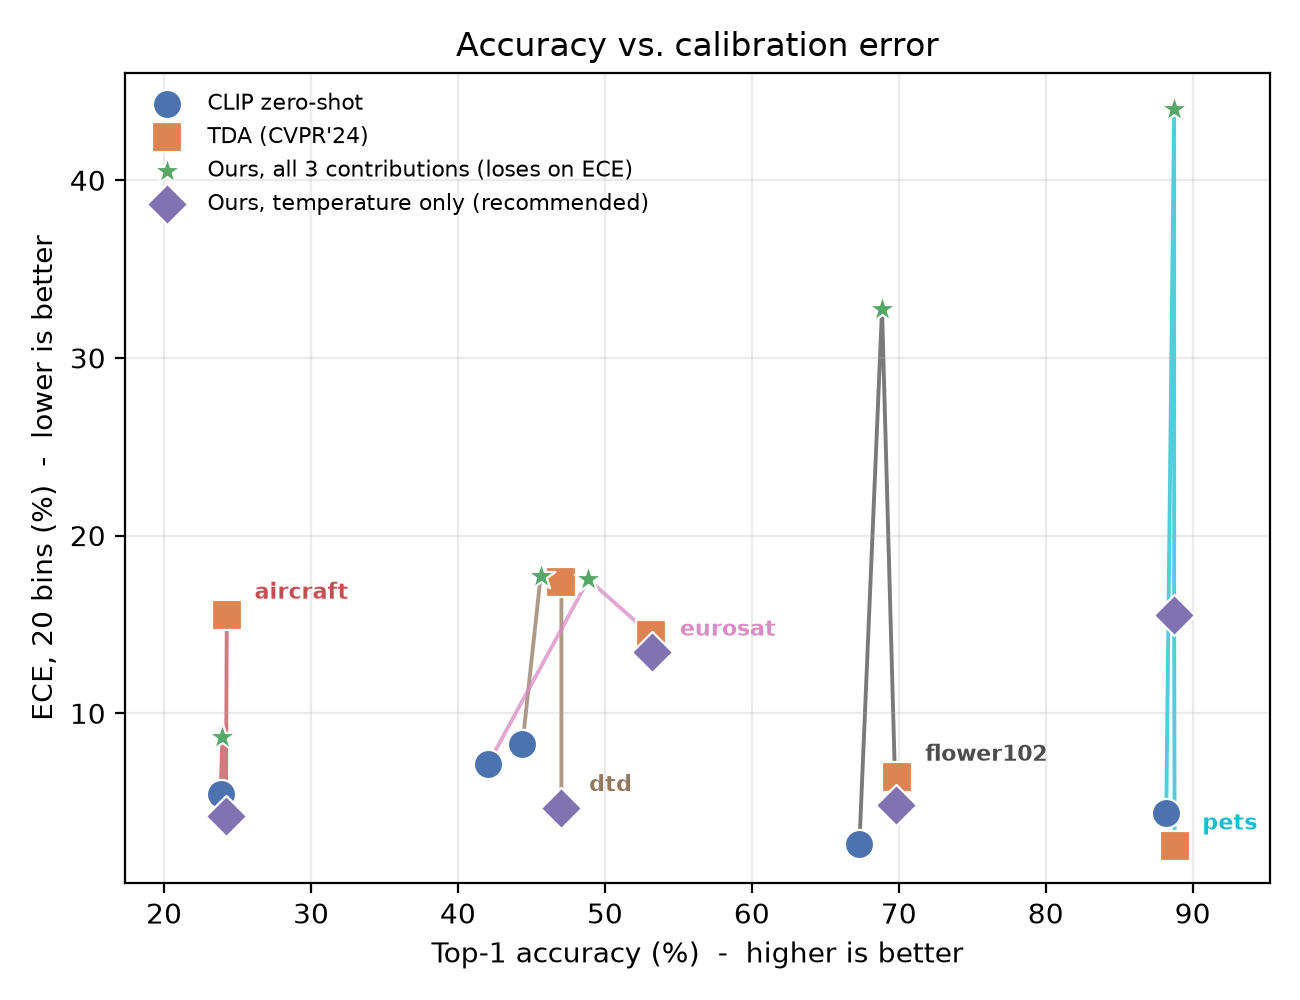
\includegraphics[width=0.75\textwidth]{accuracy_vs_ece.png}
    \caption{Accuracy vs.\ ECE, all five datasets. The purple diamond (LOO temperature only,
    Section~\ref{sec:ablation}) is the configuration this report ultimately recommends, plotted
    alongside the three headline methods. Marker shape and colour identify the method (see legend);
    each dataset's four points are joined by a line in that dataset's own colour, labelled at the
    line's right-hand end. Lines run left to right by accuracy; they mark grouping only, not a
    progression.}
    \label{fig:scatter}
\end{figure}

\subsection{Reliability diagrams}

Figure~\ref{fig:reliability} plots, per dataset, the confidence-vs-accuracy curve for each of
the three headline methods plus the ablation's \texttt{temp}-only variant (a curve on the
dashed identity line is perfectly calibrated). The
grid makes the aggregate ECE numbers in Table~\ref{tab:main} legible per bin, and the direction
of the failure is visible directly: on every dataset, \texttt{cal\_tda}'s curve sits
\emph{above} the identity line -- accuracy exceeds stated confidence, not the reverse. In
the five \texttt{cal\_tda} reliability records the highest occupied confidence bin tops out at
0.70 on EuroSAT and at 0.60 or below on the other four, so there is no high-confidence region
to be confidently wrong in; the method is instead severely \emph{underconfident}, most visibly on
Pets, where 88.74\% accuracy is reported at only 44.77\% mean confidence. Section~\ref{sec:discussion}
explains the mechanism, including why Aircraft -- the one dataset where the bundle's ECE
looked like an improvement over TDA in Table~\ref{tab:main} -- is not a case of the method
correcting itself, but the smallest instance of the same underconfidence effect.

\begin{figure}[htbp]
    \centering
    % Three panels per row. Two-per-row was tried and reverted: five square panels
    % in three rows exceed \textheight, and LaTeX responds by pushing the caption
    % and the last subcaption clean off the bottom of the paper ("Float too large
    % for page by 128pt"). On-page legibility is fixed in make_figures.py instead,
    % by shrinking the matplotlib canvas rather than enlarging the float. Slot six
    % holds the legend the five panels share.
    \begin{subfigure}[t]{0.32\textwidth}
        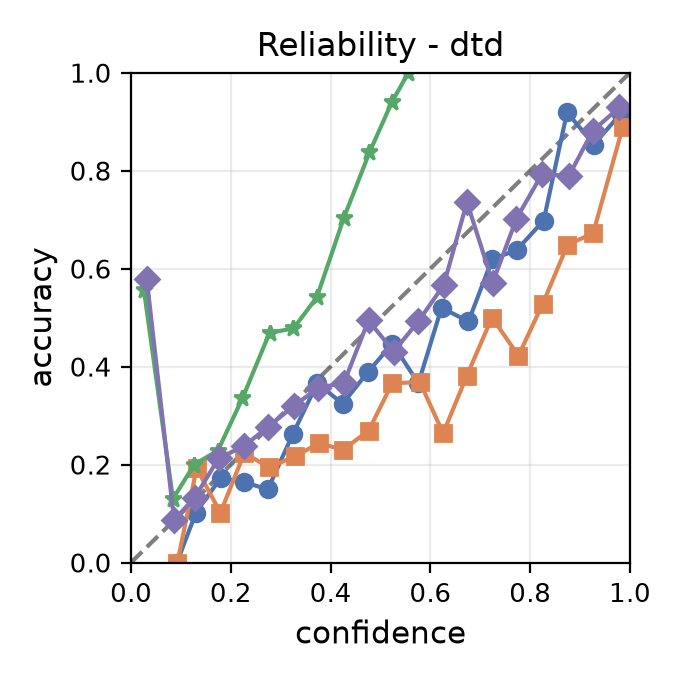
\includegraphics[width=\linewidth]{reliability_dtd.png}
        \caption{DTD}
    \end{subfigure}
    \begin{subfigure}[t]{0.32\textwidth}
        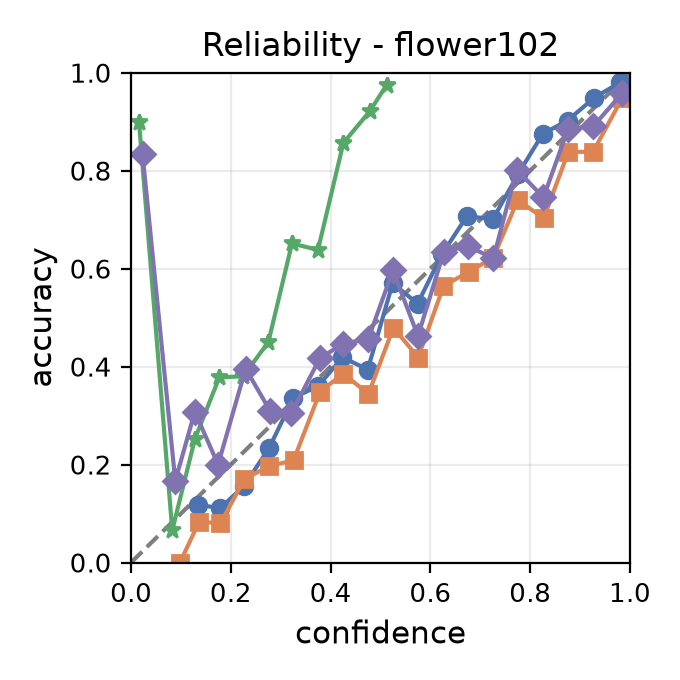
\includegraphics[width=\linewidth]{reliability_flower102.png}
        \caption{Flowers102}
    \end{subfigure}
    \begin{subfigure}[t]{0.32\textwidth}
        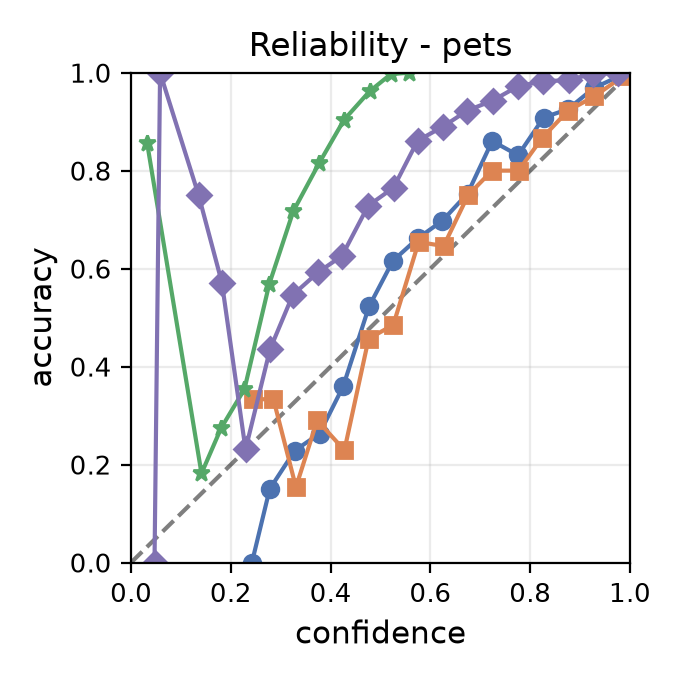
\includegraphics[width=\linewidth]{reliability_pets.png}
        \caption{Pets}
    \end{subfigure}\\[1ex]
    \begin{subfigure}[t]{0.32\textwidth}
        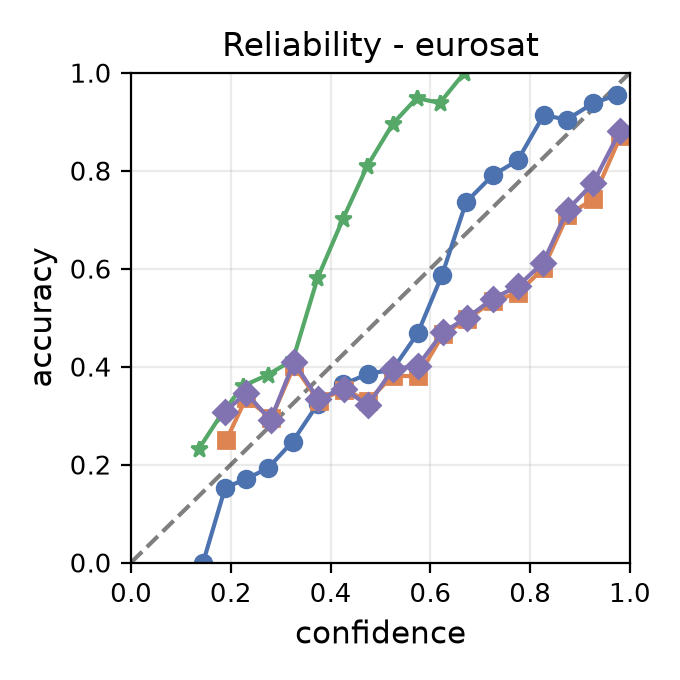
\includegraphics[width=\linewidth]{reliability_eurosat.png}
        \caption{EuroSAT}
    \end{subfigure}
    \begin{subfigure}[t]{0.32\textwidth}
        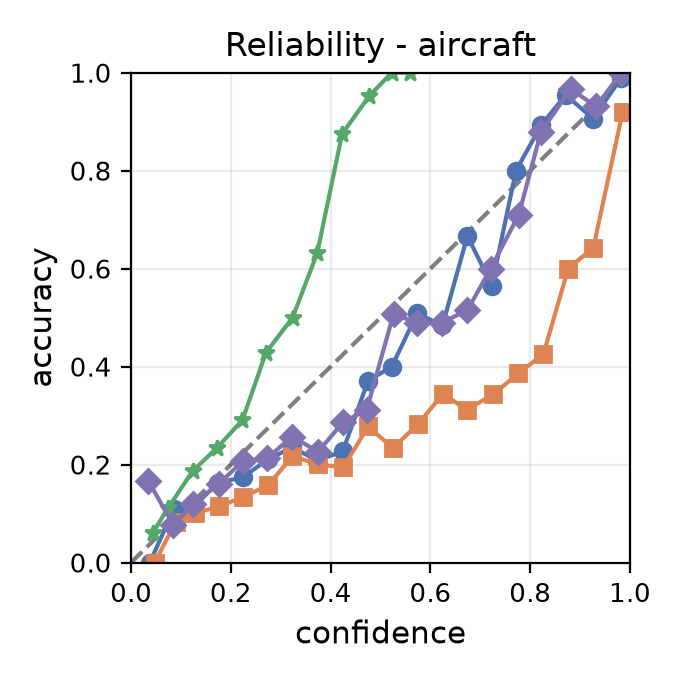
\includegraphics[width=\linewidth]{reliability_aircraft.png}
        \caption{Aircraft}
    \end{subfigure}
    % A minipage, not a subfigure: the legend is not a sixth panel and must not be
    % lettered (f) or counted in the figure's subcaptions.
    %
    % [b], not [t], and an explicit height. Given a height, minipage's [t] puts the
    % box *top* on the row's baseline -- which is the bottom edge of the panels
    % beside it, so the legend landed a full panel below the row. [b] puts the box
    % bottom there instead, so a box exactly one panel high (0.32\textwidth: the
    % panels are square) spans the row, and inner-pos c centres the legend in it.
    \begin{minipage}[b][0.32\textwidth][c]{0.32\textwidth}
        \centering
        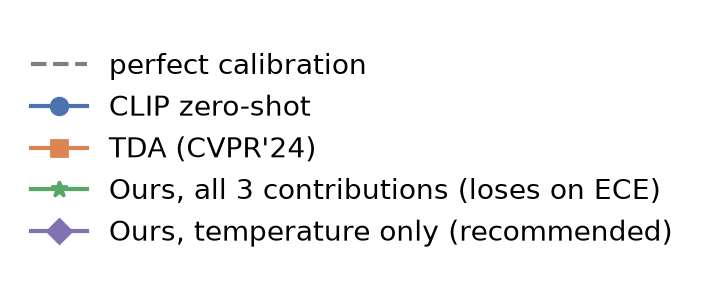
\includegraphics[width=\linewidth]{reliability_legend.png}
    \end{minipage}
    \caption{Reliability diagrams, all five datasets: zero-shot CLIP, TDA, \texttt{cal\_tda}
    (all three contributions), and the ablation's \texttt{temp}-only variant. All five panels
    share the legend at bottom right; a curve on the dashed identity line is perfectly calibrated.}
    \label{fig:reliability}
\end{figure}

\subsection{The ablation}
\label{sec:ablation}

Table~\ref{tab:ablation} (generated by \texttt{analysis/make\_ablation\_table.py} from a
40-run sweep -- all eight on/off combinations of the three contributions, on all five datasets)
isolates which of the three changes are responsible for the failure above.

\begin{table}[htbp]
\centering
\begin{tabular}{lrr}
\toprule
 & Accuracy & ECE \\
\midrule
none: TDA-equivalent (all flags off) & 56.60 & 11.28 \\
margin: + margin admission & 53.67 & 18.06 \\
fusion: + probabilistic fusion & 55.60 & 24.54 \\
temp: + LOO temperature & 56.60 & 8.54 \\
margin\_fusion: + margin + fusion & 55.22 & 23.94 \\
margin\_temp: + margin + temperature & 53.67 & 19.39 \\
fusion\_temp: + fusion + temperature & 55.60 & 24.78 \\
all: all three (ours) & 55.22 & 24.12 \\
\bottomrule
\end{tabular}
\caption{Ablation: mean accuracy and ECE (\%) across the five datasets.}
\label{tab:ablation}
\end{table}


\textbf{Contribution 3 (LOO temperature scaling) alone succeeds.} The ablation's own \texttt{none} baseline is
\texttt{cal\_tda} with all three flags off, run inside the same 40-run sweep; it is the correct
same-code-path comparison, since \texttt{temp} and \texttt{none} differ by exactly one config
flag. Against it, \texttt{temp} matches accuracy \emph{exactly}, to 0.00 points, on all five
datasets -- a structural guarantee, since temperature scaling is a monotonic rescaling of the
logits and cannot change an argmax. It cuts mean ECE from 11.28\% to 8.54\%, the best mean ECE
of all eight ablation variants, including \texttt{all} (24.12\%). The per-dataset breakdown is in Table~\ref{tab:temp-per-dataset}:

\begin{center}
\begin{tabular}{lrrr}
\toprule
Dataset & \texttt{none} ECE & \texttt{temp} ECE & Change \\
\midrule
Aircraft   & 15.56 & 4.21  & $-11.35$ \\
DTD        & 17.41 & 4.68  & $-12.73$ \\
EuroSAT    & 14.43 & 13.43 & $-1.00$ \\
Flowers102 & 6.51  & 4.85  & $-1.66$ \\
% \textbf does not reach inside math mode, so $+13.06$ printed at roman weight
% next to a bold "(worse)" in the same cell. \mathbf carries the weight in.
Pets       & 2.48  & \textbf{15.54} & \textbf{$\mathbf{+13.06}$ (worse)} \\
\bottomrule
\end{tabular}
\captionof{table}{Per-dataset ECE (\%) for the ablation's \texttt{none} and \texttt{temp} variants. Pets is the one reversal.}
\label{tab:temp-per-dataset}
\end{center}

This is not a uniform win: on Pets, where the \texttt{none} baseline was already very well
calibrated (2.48\% ECE),
LOO temperature scaling makes calibration substantially \emph{worse}. We discuss the mechanism
in Section~\ref{sec:discussion} rather than average it away.

\textbf{Two counts, and why they differ.} Against the ablation's \texttt{none} baseline,
\texttt{temp} meets the spec's success criterion on \textbf{4 of 5} datasets (all but Pets).
Against the separately run headline \texttt{tda} rows in Table~\ref{tab:main}, the count is
lower -- \textbf{2 of 5} -- because \texttt{none} and \texttt{tda} are two different process
invocations of what should be identical logic, and in practice differ by 0--4 flipped
predictions per dataset out of 1{,}692--8{,}100 samples. The cause is not a logic difference:
upstream \texttt{tda} accumulates its final logits in fp16, while \texttt{cal\_tda} (even
with every flag off) upcasts to fp32 before its final step, and at CLIP's logit magnitudes that
rounding difference is worth roughly one unit in the last place -- enough, on
borderline-margin predictions, to flip an argmax once every few hundred to a few thousand
samples. Both counts are correct; they
answer different questions. The 4-of-5 count answers whether temperature scaling, holding
everything else fixed, helps calibration without moving accuracy -- yes, on 4 of 5. The
2-of-5 count answers whether a \texttt{temp}-only run, as a real separate process, beats the
specific \texttt{tda} numbers quoted in Table~\ref{tab:main} -- only on 2 of 5, because of run-to-run floating-point drift that
is two orders of magnitude smaller than any effect discussed above.

\textbf{Contributions 1 and 2 are the ones actually responsible for the bundle's failure.}
Margin admission alone \emph{lowers} mean accuracy (56.60\% $\rightarrow$ 53.67\%) and raises
mean ECE (11.28\% $\rightarrow$ 18.06\%): its selectivity throws away cache signal the
unfiltered cache was using correctly on some datasets. Probabilistic fusion alone is the worst
single component: it raises mean ECE to 24.54\%, driven by blowups on Flowers102 (32.46\%) and
Pets (43.77\%) specifically, though it happens to help Aircraft (15.56\% $\rightarrow$
9.16\%) -- the reason ``all three'' still beats plain TDA's ECE on that one dataset. Neither
contribution helps consistently even in isolation; both actively hurt the mean.

Cache admission rates, which explain part of why margin admission behaves so differently across
datasets, are reported in Section~\ref{sec:admission-rates}.

\section{Discussion}
\label{sec:discussion}

\subsection{Where it worked, and why}

LOO temperature scaling alone is a real, if not universal, calibration improvement. The
mechanism is direct: it always smooths the model's confidence toward a single label-free
accuracy estimate computed from the cache. Where TDA's cache was badly overconfident relative
to its own accuracy -- DTD (17.41\% $\rightarrow$ 4.68\% ECE) and Aircraft (15.56\%
$\rightarrow$ 4.21\%, same-code-path \texttt{none}-vs-\texttt{temp} comparison) chief among
them -- pulling confidence down toward the estimate is exactly the correction needed, and the
improvement is large.

\subsection{Where it did not, and why}

The same mechanism explains the Pets reversal. On Pets, TDA's cache was already close to
perfectly calibrated (2.52\% ECE for the headline \texttt{tda} run, 2.48\% for the ablation's
\texttt{none} baseline) -- the model's stated confidence already matched its
accuracy. LOO temperature scaling has no notion of ``already well calibrated''; it always
smooths toward the LOO estimate regardless of how good the starting point was, so with no
overconfidence to correct, it manufactures underconfidence instead (ECE rises to 15.54\% under
\texttt{temp}, or as high as 43.98\% under the full bundle). A method that only ever pushes
confidence toward one estimate, with no mechanism to detect when the starting point does not
need correcting, will help wherever that estimate happens to be closer to the truth than the
model's own confidence, and hurt wherever the estimate is not.

Margin admission and probabilistic fusion fail for related but distinct reasons. Margin
admission's single global threshold (\texttt{margin\_threshold} $= 1.0$) is not portable:
measured admission rates (Section~\ref{sec:admission-rates}) run from 15.9\% on Aircraft to
81.9\% on Pets, and they track zero-shot CLIP's accuracy rather than class count. On Aircraft the cache
mostly starves; on Pets the gate is nearly a no-op. The gate is therefore most selective exactly
where the cache had the most to contribute. Neither
extreme is what a per-dataset-tuned gate would look like, and, as Section~\ref{sec:results} shows, its
selectivity costs accuracy outright (56.60\% $\rightarrow$ 53.67\% under margin admission
alone).

Probabilistic fusion, meanwhile, is the single worst component in the ablation (mean ECE
24.54\%) -- but not for the reason it first appears. \texttt{compute\_cache\_logits}
(inherited unmodified from upstream TDA) returns, for each class, a sum of
$\exp(-\beta(1 - \mathrm{affinity}))$ terms over whatever cached items belong to that class --
an unnormalized, comparatively small-magnitude quantity, since affinity is a cosine similarity
in $[-1, 1]$ and only the handful of classes actually represented in a small cache get a
nonzero score at all. $\sigma(z_{\text{cache}})$ is therefore close to uniform relative to
$\sigma(z_{\text{clip}})$, which is sharply peaked because CLIP's own logits are already scaled
by its learned logit scale ($\approx 100$). Averaging a near-uniform distribution into a
near-one-hot one at $w = 0.5$ (Eq.~\eqref{eq:fusion}) caps top-1 probability well below what CLIP
alone would report, \emph{regardless of how much evidence actually supports the prediction} -- fusion
does not need both sources to agree on a wrong answer to produce this effect; it produces the effect on
every sample, right or wrong alike. This single fact accounts for everything the reliability
diagrams show (Section~\ref{sec:results}): no \texttt{cal\_tda} reliability record on any
dataset reaches even 0.70 mean confidence in its highest-occupied bin, mean confidence sits
8.7--44 points below accuracy on every dataset, and the size of that gap tracks accuracy itself:
it is largest on the highest-accuracy dataset (Pets, 88.74\% accuracy capped near 44.77\%
confidence) and smallest on the lowest-accuracy one (Aircraft, 23.97\% accuracy capped near
15.32\%). That is what a fixed confidence ceiling does -- it costs a high-accuracy dataset far
more calibration error than a low-accuracy one. Fusion's ECE is therefore not overconfidence from agreeing wrong
answers; it is underconfidence manufactured by capping every prediction's confidence near one
fixed point, independent of correctness.

This also explains Aircraft's apparent improvement in Table~\ref{tab:main} without invoking any
real correction. The \texttt{none} baseline on Aircraft is overconfident to begin with (mean
confidence 39.77\% against 24.21\% accuracy, ECE 15.56\%) -- ordinary TDA-style overconfidence.
Adding fusion does not fix that overconfidence; it overshoots straight past it, capping
confidence at 15.2--15.4\% against 23.97--24.42\% accuracy (ECE 8.65--9.20\%). The resulting
ECE is smaller purely because Aircraft's true accuracy (23.97\%) happens to sit close to
fusion's confidence ceiling on this particular dataset -- an accident of
where the ceiling landed relative to Aircraft's accuracy, not evidence that fusion diagnosed and
corrected \texttt{none}'s overconfidence. On every other dataset, where accuracy is higher, the
same ceiling produces a much larger gap in the other direction, which is why fusion is the worst
component overall despite this one favourable-looking case.

\subsection{The margin$\times$temperature interaction, and its limits}

An earlier single-dataset (DTD) observation suggested a clean interaction, and the five-dataset
runs bear it out: once margin
admission and fusion are both active, the LOO temperature search pins at its grid boundary
$T = 1.0$ on 98--100\% of samples on every dataset, meaning the search wants to sharpen further
than the smoothing-only grid allows and Contribution 3 becomes effectively inert on top of Contributions 1
and 2 -- consistent with the ECE difference between \texttt{margin\_fusion} and \texttt{all}
being tiny everywhere (0.00--0.36 points). Testing that story against temperature on top of
margin \emph{alone} (without fusion in between) shows it does not generalize cleanly: pinning
drops to 75--95\% on four datasets, with a correspondingly larger ECE effect (DTD improves by
2.81 points, Flowers102 by 2.25), and \textbf{Pets breaks the pattern outright} -- its
\texttt{margin\_temp} run pins only 0.2\% of samples at the boundary, the opposite of inert, and
it is exactly on Pets, already well calibrated under margin alone (2.53\% ECE), that adding
temperature does the most damage of any margin-plus-temperature run (2.53\% $\rightarrow$
14.79\%; the larger temperature-induced regression in the ablation is Pets without margin,
Table~\ref{tab:temp-per-dataset}: 2.48\% $\rightarrow$ 15.54\%). The
single-dataset story pointed to one mechanism; five datasets show it holds strongly with fusion
present, holds more weakly for margin alone, and inverts on the one dataset a single-dataset
study would have missed. We report this as a caution about generalizing a mechanism from one
dataset, not as a discarded finding -- the underlying explanation (temperature is inert exactly
when the search is already pinned against its floor) still holds; what changes across datasets
is how often that precondition is met.

\subsection{Accuracy/calibration trade-off, stated plainly}

None of the three contributions, alone or combined, is a free lunch. Contribution 3 is the one
change in this project that costs nothing in accuracy (it structurally cannot, being a
monotonic rescaling) and buys a real mean calibration improvement -- but even that
improvement is not uniform, and reverses on the one dataset that was already well calibrated.
Contributions 1 and 2 cost accuracy, calibration, or both, on average, and the one apparent
exception -- fusion's lower ECE on Aircraft -- is not a benefit either, once its mechanism is
understood: it is the same confidence-capping failure landing, by the accident of that one
dataset's low accuracy, closer to correct than the overconfidence it replaced. The honest summary of this project's
central finding is that a training-free, label-free calibration fix is achievable, but it is one
targeted change (temperature scaling on a label-free accuracy estimate), not the three-part
bundle we set out to build.

\section{Conclusion}

This project set out to undo TDA's calibration loss with three training-free, label-free
changes to its cache loop, and measured whether that worked rather than assuming it. It did not:
bundled together as specified, the three contributions meet the project's own success criterion
on 0 of 5 datasets, trading away both accuracy and calibration relative to plain TDA. But the
ablation that made this failure legible also isolated a real success inside it -- leave-one-out
temperature scaling, run alone, matches TDA-equivalent accuracy exactly while cutting mean ECE
by 24\% toward zero-shot CLIP's level, and meets the success criterion on 4 of 5 datasets, for
a structural reason (a monotonic
rescaling cannot move accuracy) that makes the result as close to guaranteed-safe as a
calibration intervention gets. Margin admission and probabilistic fusion, the other two
contributions, are the ones actually responsible for the bundle's failure, and neither helps
consistently even in isolation. The finding this report stands behind is therefore narrower and
more specific than the one we set out to demonstrate: not ``three changes fix TDA's
calibration,'' but ``one of three does, and we now know which, and why the other two do not.''


\bibliographystyle{plainnat}
\bibliography{refs}
\end{document}
